
\section{Vektorer og vektorfunktioner}

Forklar om vektorer og vektorfunktioner, herunder hvordan de differentieres.

\subsection{Bevis af cirklens parameterfremstilling}

\begin{proofw}
    \begin{figure}[h]
        \centering
        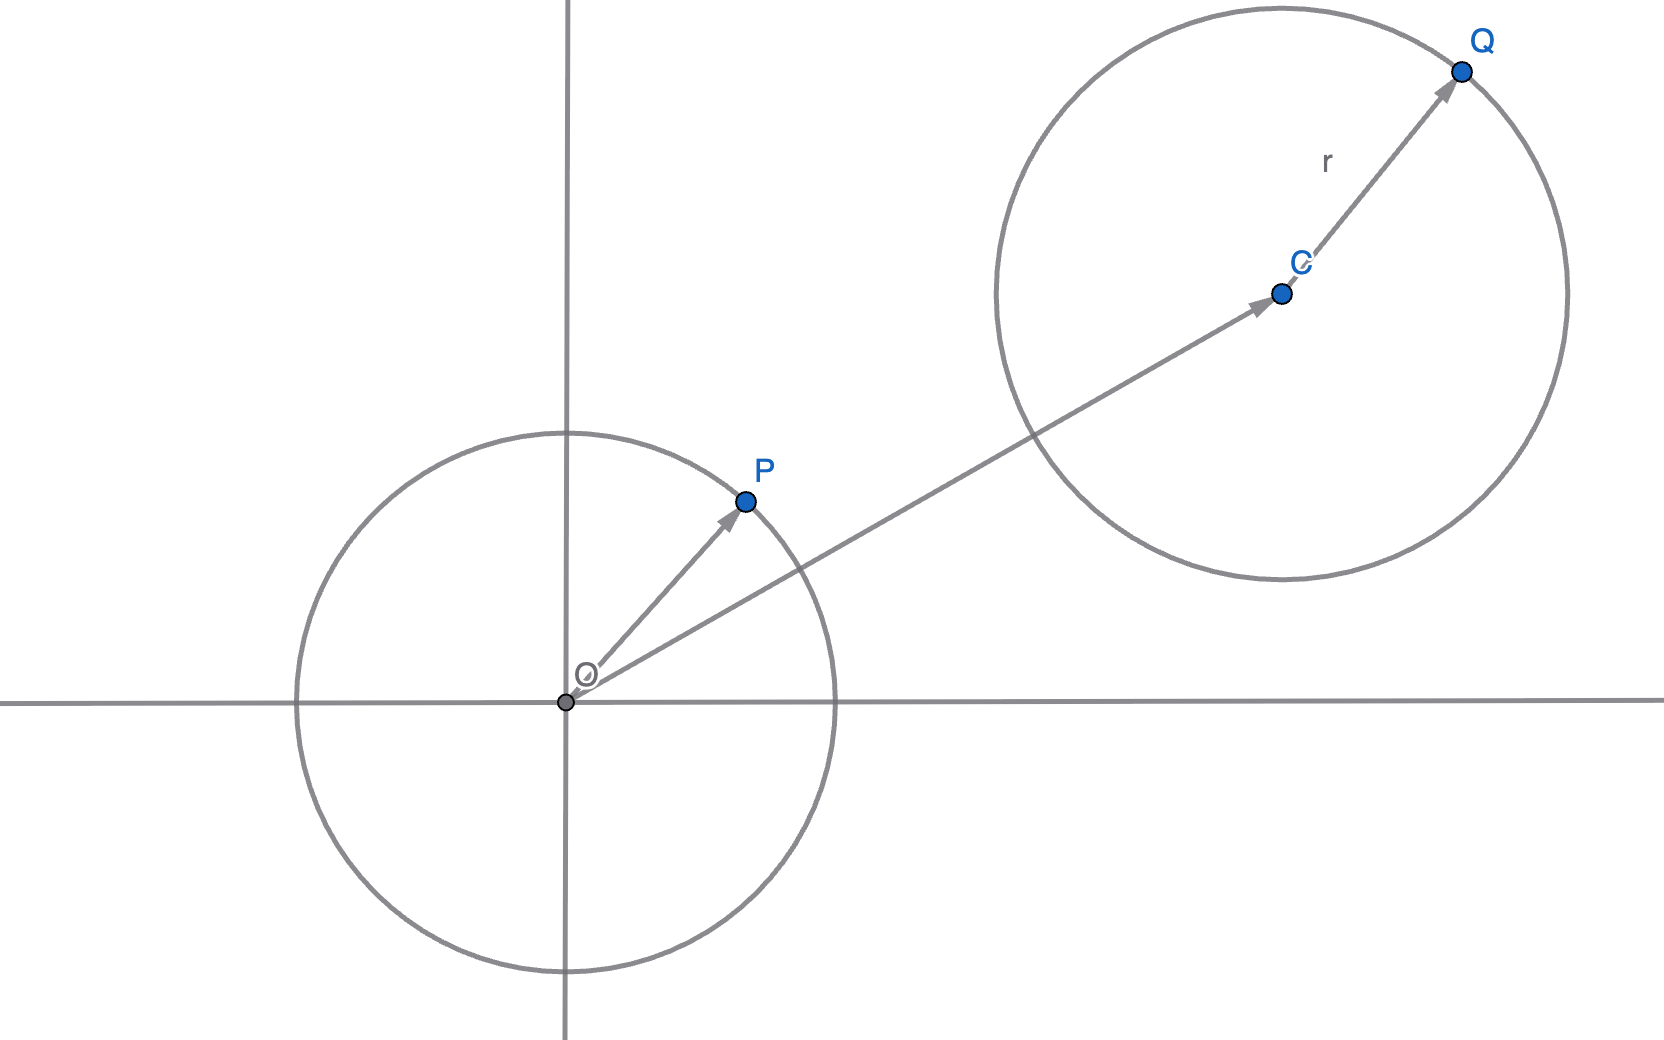
\includegraphics[scale=0.3]{skitser/cirkel.png}
    \end{figure}

    Betragt ovenstående figur, først tager vi tilfældet,
    hvor cirklen har centrum i origo. Her vil alle punkter
    på cirkelperifirien kunne beskrives som en skalering af enhedscirklen, derfor:

    $$
        \vec{OP}=\begin{pmatrix}
            r\cdot \cos(t)
            \\
            r\cdot \sin(t)
        \end{pmatrix}
    $$
    
    For cirklen, der ikke har centrum i origo, er situationen en smule anderledes,
    men vektoren $\vec{CQ}=\vec{OP}$, da cirklerne har samme radius $r$.
    Vi anvender indskudsreglen til at finde:

    $$
        \vec{OQ}=\vec{OC}+\vec{CQ}
    $$

    Disse værdier kender vi, så parameterfremstillingen bliver:

    $$
    \begin{pmatrix}
        x \\ y
    \end{pmatrix}
    =\begin{pmatrix}
        a \\ b
    \end{pmatrix}
    +
    \begin{pmatrix}
        r \cdot \cos(t)
        \\
        r \cdot \sin(t)
    \end{pmatrix}
    =\begin{pmatrix}
        a+ r \cdot \cos(t)
        \\
        b+ r \cdot \sin(t)
    \end{pmatrix}
    $$

\end{proofw}
